%===================================================
\chapter{Gravitational Perturbations and the Geopotential Model}
\label{app:geopotential}
%===================================================

The Keplerian elements $\vec{A}_k$ (Eq.~\ref{eq:orbital_state_vector}) describe two-body motion under the idealised potential $U_0 = \mu/r$, which assumes a perfectly spherical, homogeneous Earth. In practice, Earth's  rotation produces an equatorial bulge of approximately 21\,km relative to the polar radius, making the geoid an oblate spheroid, as seen in Fig. \ref{fig:earth_oblatenes}. As a consequence, the gravitational potential becomes a function of both geocentric latitude $\varphi_{Gc}$ and longitude $\lambda$, and the realist acceleration acting on satellite $S_k$ deviates from the trajetory prediction from the Keplerian model. This appendix establishes the analytical gravitational potential model \cite{valladoFundamentalsAstrodynamicsApplications2001}, which serves as the foundation for defining orbital perturbation effects exploited by orbit types such as Sun-Synchronous Orbit (SSO, Appendix~\ref{app:sso_orbit}) and Repeating Ground Track Orbit (RGTO). The secular perturbation rates derived from this model---specifically the $J_2$-driven drift rates $\dot{\Omega}$, $\dot{\omega}$, and $\dot{M}$---are the key results used in the main text (Sec.~\ref{sec:perturbed_orbital_elements}) to establish the RGTO resonance condition.

\begin{figure}[H]
    \centering
    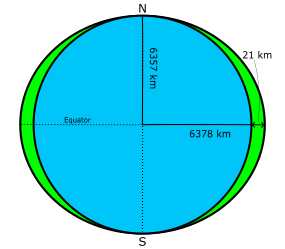
\includegraphics[width=0.4\linewidth]{images/oblateearth.png}
    \caption{\footnotesize{Exaggerated depiction of Earth's oblate shape. The equatorial radius exceeds the polar radius by approximately 21\,km, breaking the spherical symmetry of the gravitational potential $U_0 = \mu/r$. \cite{J2Perturbation}}}
    \label{fig:earth_oblatenes}
\end{figure}

The gravitational potential exterior to the Earth is modelled by an infinite series of spherical harmonics, each term representing a deviation from the uniform spherical case \cite{valladoFundamentalsAstrodynamicsApplications2001}:
\begin{equation}
    U(r, \varphi_{Gc}, \lambda) \;=\; \frac{\mu}{r}
    \left[
        1 + \sum_{L=2}^{\infty} \sum_{M=0}^{L}
        \left( \frac{R_{\oplus}}{r} \right)^{\!L}
        P_{LM}(\sin \varphi_{Gc})\,
        \bigl(
            C_{LM} \cos M\lambda + S_{LM} \sin M\lambda
        \bigr)
    \right],
    \label{eq:geopotential}
\end{equation}
where $r$ is the geocentric distance of $S_k$, $R_{\oplus}$ is Earth's reference equatorial radius, $P_{LM}$ are the associated Legendre polynomials of degree $L$ and order $M$, and $C_{LM}$, $S_{LM}$ are the normalised harmonic coefficients determined empirically from satellite tracking and gravimetry missions. The index pair $(L, M)$ classifies each term by the spatial structure it encodes:
\begin{itemize}
    \item \textbf{Zonal} ($M = 0$): axially symmetric, latitude-dependent only; encode Earth's flattening ($J_2$, $J_3$, \ldots).
    \item \textbf{Sectoral} ($L = M$): longitude-dependent, symmetric about the equatorial plane.
    \item \textbf{Tesseral} ($L \neq M$,\; $M \neq 0$): mixed latitude--longitude variations, encoding the ``lumpy'' mass distribution.
\end{itemize}

\begin{figure}[H]
    \centering
    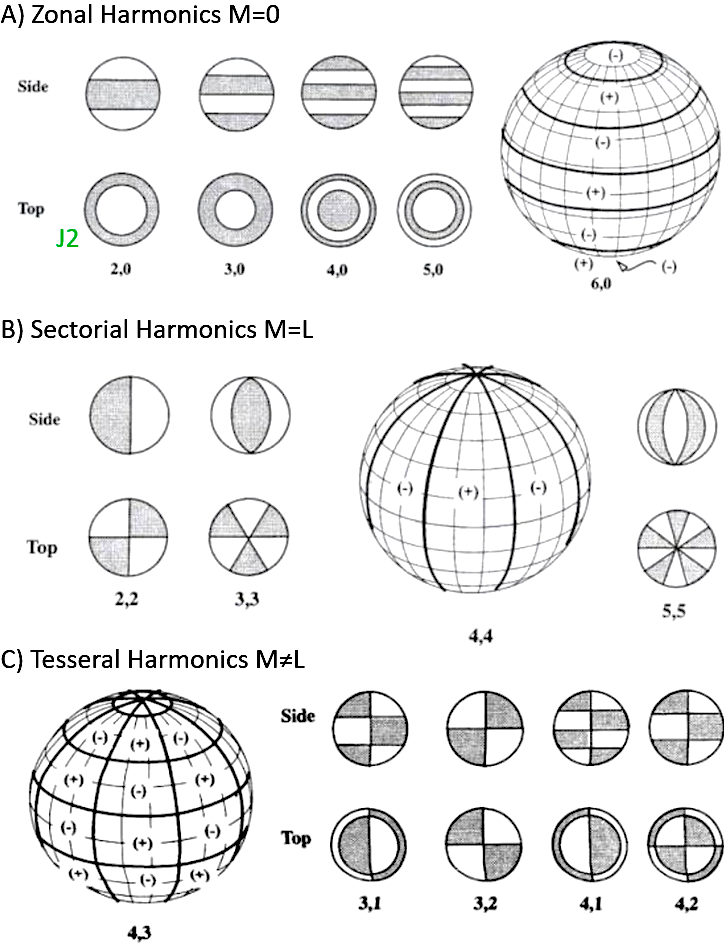
\includegraphics[width=0.5\linewidth]{images/geopotencial_harmonics.png}
    \caption{\footnotesize{Zonal ($M=0$), sectoral ($L=M$), and tesseral ($L \neq M$, $M\neq 0$) spherical harmonic modes of the geopotential. Increasing degree $L$ and order $M$ subdivide the sphere into progressively finer latitude and longitude bands. \cite{lgeorge2Chapter10Orbital, valladoFundamentalsAstrodynamicsApplications2001}}}
    \label{fig:geopotential_harmonics_zonal_sectorial_tectral}
\end{figure}

%===================================================
\section{The Dominant \texorpdfstring{$J_2$}{J2} Perturbation}
\label{sec:j2pert}
%===================================================

Among all harmonic terms in Eq.~\ref{eq:geopotential}, the second zonal coefficient $J_2 \equiv -C_{20} \approx 1.08263 \times 10^{-3}$ is by far the largest, exceeding the next significant coefficient by approximately three orders of magnitude (Table~\ref{tab:harmonic_coefficients}). It quantifies the oblateness that is already visible in Fig.~\ref{fig:earth_oblatenes}. Using only this term, Eq.~\ref{eq:geopotential} reduces to the $J_2$-perturbed potential:
\begin{equation}
    U_{J_2}(r,\theta) \;=\; \frac{\mu}{r}\left[
        1 - J_2 \left(\frac{R_{\oplus}}{r}\right)^{\!2} P_2(\cos\theta)
    \right],
    \label{eq:potential_j2}
\end{equation}
where $P_2(\cos\theta) = \tfrac{1}{2}(3\cos^2\theta - 1)$ is the second Legendre polynomial and $\theta$ is the colatitude.

\begin{table}[H]
\centering
\caption{\footnotesize{Representative values of the dominant geopotential harmonic coefficients. $J_n \equiv -C_{n0}$ are the zonal coefficients; $C_{LM}$, $S_{LM}$ are tesseral/sectoral coefficients. $J_2$ exceeds all others by approximately three orders of magnitude. \cite{valladoFundamentalsAstrodynamicsApplications2001}}}
\label{tab:harmonic_coefficients}
\begin{tabular}{lll}
\toprule
Coefficient & Value & Physical description \\
\midrule
$J_2$            & $\phantom{-}1.08263 \times 10^{-3}$  & Dominant equatorial bulge (oblateness)     \\
$J_3$            & $-2.532 \times 10^{-6}$               & Pear-shaped north--south asymmetry         \\
$J_4$            & $-1.620 \times 10^{-6}$               & Higher-order zonal correction              \\
$J_5$            & $-2.277 \times 10^{-7}$               & Higher-order zonal variation               \\
$J_6$            & $\phantom{-}5.406 \times 10^{-7}$     & Further refinement of Earth's shape        \\
$C_{22}$         & $\phantom{-}1.574 \times 10^{-6}$     & Sectoral: equatorial ellipticity           \\
$S_{22}$         & $-1.867 \times 10^{-6}$               & Sectoral variation                         \\
$C_{21},\,S_{21}$& ${\sim}1 \times 10^{-6}$              & Tesseral terms (low degree/order)          \\
\bottomrule
\end{tabular}
\end{table}

\begin{figure}[H]
    \centering
    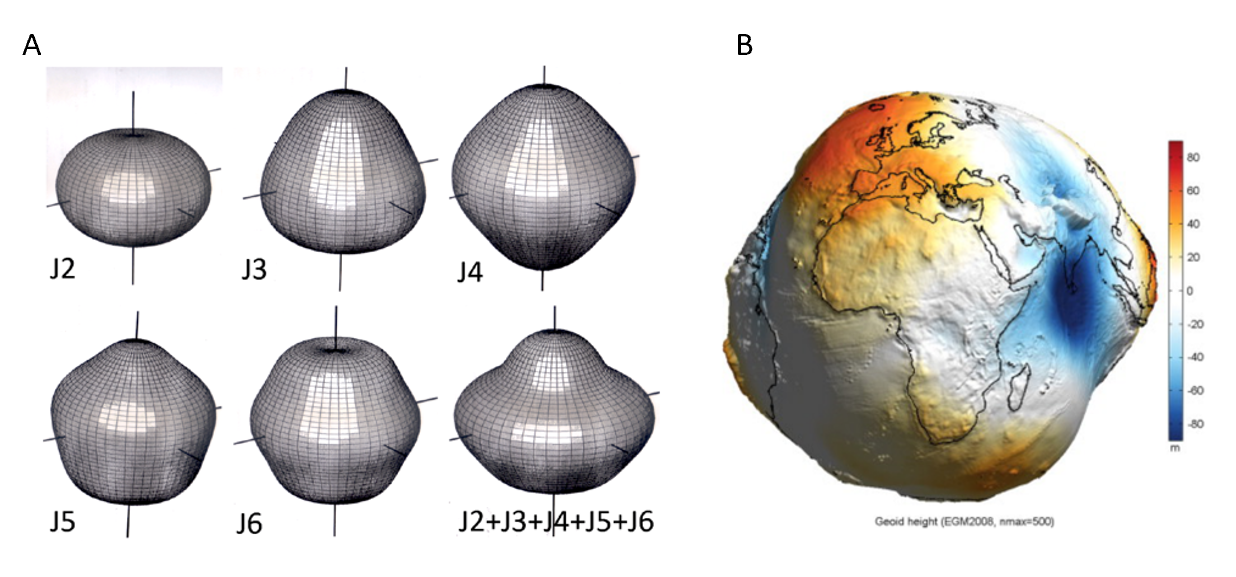
\includegraphics[width=0.5\linewidth]{images/geoid_gravitational_Example_hamoci_comparation.png}
    \caption{\footnotesize{Left: spatial patterns for selected harmonic degrees. Right: geoid height relative to the EGM2008 gravitational field model \cite{barnesEarthGravitationalModel2015}, produced using over 2000 harmonic coefficients. The $J_2$ contribution dominates the large-scale structure; higher-order terms refine local variations. \cite{lgeorge2Chapter10Orbital}}}
    \label{fig:geoid_Graviational_example_harmonics_comparation}
\end{figure}
